%%%%%%%%%%%%%%
% ch3 : cristallographie % 
%%%%%%%%%%%%%%

\chapter{L'état cristallin et l'état amorphe}
\section{Introduction}
	\begin{wrapfigure}[6]{l}{5cm}
	\vspace{-6mm}
	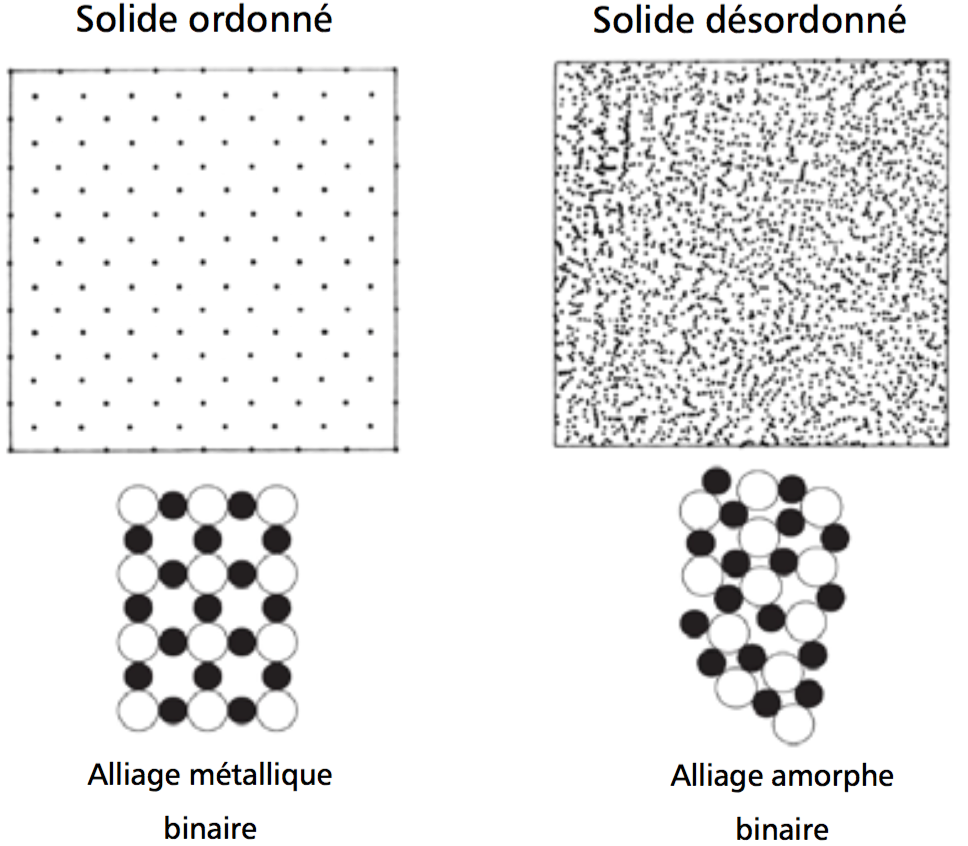
\includegraphics[scale=0.28]{ch3/1}
	\end{wrapfigure}
	Un solide cristallin (ordonné) est caractérisé par un ordre sur de longues distances alors qu'un solide amorphe (désordonné) ou vitreux se caractérise par l'absence d'ordre. Les métaux et les céramiques sont cristallins. Des températures de refroidissement extrêmes depuis l'état fondu peuvent donner lieu à des métaux amorphes pour des alliages assez complexes.\\\\\\
	
	\begin{wrapfigure}[6]{r}{3cm}
	\vspace{-10mm}
	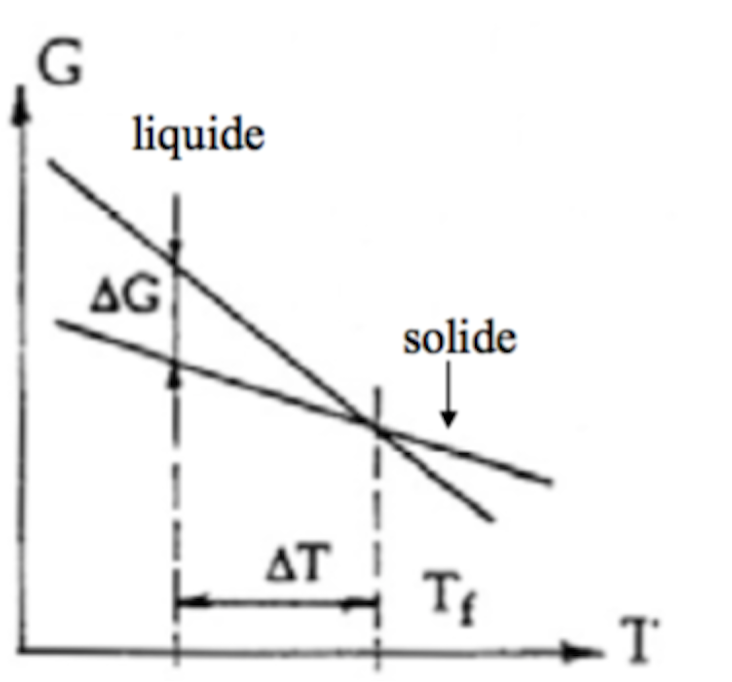
\includegraphics[scale=0.25]{ch3/2}
	\end{wrapfigure}
	La thermodynamique nous apprend qu'à pression constante, l'état d'équilibre correspond au minimum de l'\textbf{enthalpie libre de Gibbs}
	\begin{equation}
		G = H-TS
	\end{equation}
	On sais alors qu'à \textbf{haute température}, l'enthropie du liquide étant plus grande que celle du solide (plus de désordre dans le liquide), la composante enthropique va l'emporter et le liquide aura une énergie libre plus faible $\rightarrow$ stable.\\
	Au contraire, à basse température, c'est l'enthalpie qui prend le dessus et est lié au rassemblement des molécules sous l'effet des forces de liaison qui entraîne sa diminution $\rightarrow$ solide.\\
	 A une température $T_f$, l'énergie des deux phases sont égales, c'est la température de fusion. 
	 
	\begin{wrapfigure}[7]{l}{3.7cm}
	\vspace{-5mm}
	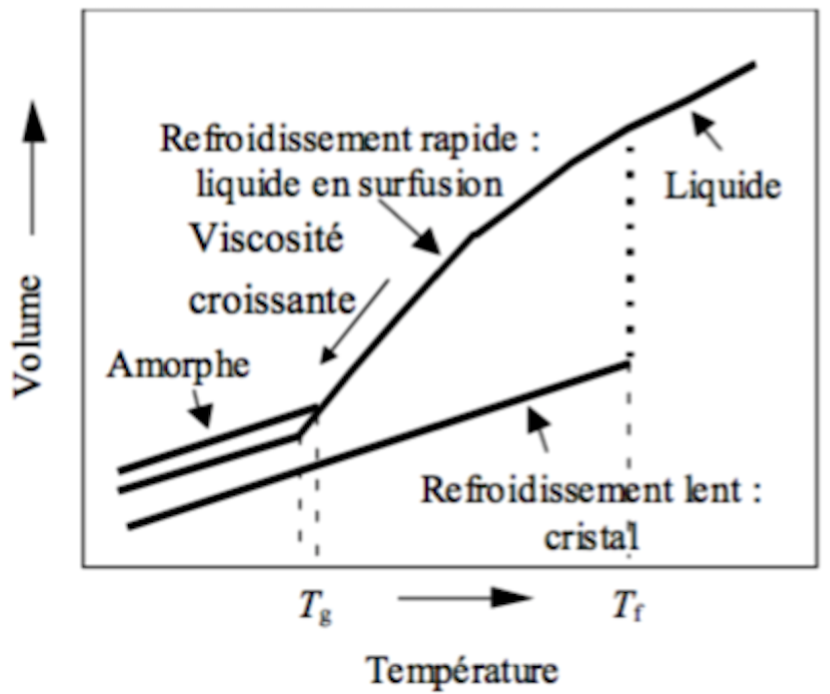
\includegraphics[scale=0.25]{ch3/3}
	\end{wrapfigure}
	Le volume d'un liquide quelconque augmente avec la température en raison de l'agitation thermique qui fait monter la distance entre les atomes ou molécules. En refroidissant lentement le liquide, on observera à la température de fusion une contraction du volume qui traduit la \textbf{mise en ordre} des atomes. Ils adoptent un empilement ordonné bien plus compact de manière à produire l'enthalpie de liaison (négative) la plus grande. Le solide sera à l'état \textbf{cristallin}.\\
	
	Lorsque la vitesse de refroidissement augmente, la contraction démarre à une \textbf{température plus basse.} Pour les longues chaînes polymétriques ou des silicates complexes (systèmes complexes), la forme stable est une forme cristalline à basse température, mais la mise en place est tellement complexe qu'un refroidissement rapide l'en empêche. Dans ce cas, lorsque la température diminue, la viscosité du liquide augmente et peut aller jusqu'à une température en dessous de laquelle l'agitation thermique n'est plus suffisante pour permettre le mouvement des atomes. Le liquide se fige alors et forme un solide en gardant la structure désordonnée du liquide $\rightarrow$ \textbf{amorphe}. La température à laquelle le liquide se fige est appelé \textbf{température de transition vitreuse} $\mathbf{T_g}$.
	
\section{Les cristaux métalliques}
\section{Les cristaux ioniques}
\section{Les cristaux covalents}
\section{La structure des polymères}